% Copyright 2015, 2016 Dustin Lang (U Toronto).
% All rights reserved.

% TO-DO:
% - Compare speed & accuracy vs galsim ?  Eg, on a Gaussian profile as
%   it goes from ~ well-sampled to undersampled
%   (pixel space vs analytic in galsim?)

\documentclass[11pt,preprint]{aastex}
\usepackage{amssymb,amsmath,mathrsfs,color}
\usepackage{bm}
\usepackage{hyperref}
\usepackage{multirow}
\usepackage{color}
\usepackage{array}
\usepackage{dcolumn}

\hypersetup{pdftitle={},
pdfauthor={Dustin Lang},pdfsubject={Astronomical image processing}}

\newcommand{\arxiv}[1]{\href{http://arxiv.org/abs/#1}{arXiv:#1}}

\newcommand{\foreign}[1]{\emph{#1}}
\newcommand{\etal}{\foreign{et\,al.}}
\newcommand{\ie}{\foreign{i.e.}}
\newcommand{\figref}[1]{\figurename~\ref{#1}}
\newcommand{\Figref}[1]{\figref{#1}}
\newcommand{\appref}[1]{Appendix \ref{#1}}
\newcommand{\eqnref}[1]{Equation \ref{#1}}
\newcommand{\niceurl}[1]{\href{#1}{\textsl{#1}}}
\newcommand{\project}[1]{\textsl{#1}}
\newcommand{\conv}{\otimes}
\newcommand{\trick}{method}
\newcommand{\Trick}{Method}

\newcommand{\CD}{C\!D}

\definecolor{gray}{rgb}{0.5,0.5,0.5}
\newcommand{\gray}[1]{\textcolor{gray}{#1}}

\slugcomment{To be submitted to The Astronomical Journal}

\keywords{methods: data analysis --- surveys --- techniques: image processing}

\begin{document}

\title{A \trick\ for fast galaxy--PSF convolution}
\author{Dustin~Lang\altaffilmark{1,2,3}}
\altaffiltext{1}%
{Dunlap Institute and Department of Astronomy \& Astrophysics,
  University of Toronto,
  50 Saint George Street, Toronto, ON, M5S 3H4, Canada}
\altaffiltext{2}%
{Visitor, Department of Physics \& Astronomy,
  University of Waterloo,
  200 University Avenue West,
  Waterloo, ON, N2L 3G1, Canada}
\altaffiltext{3}%
{dstndstn@gmail.com}
\date{DRAFT \today}
\shorttitle{Fast Galaxy--PSF Convolution}
\shortauthors{Lang}

\begin{abstract}
  I present a \trick\ for the fast convolution of a model galaxy
  profile by a point-spread function (PSF) model 
  %that can be represented in the Fourier domain.
  represented as a pixel grid.
  The \trick\ relies upon two
  observations: First, most simple galaxy profiles of common interest
  (deVaucouleurs, exponential, S\'ersic) can be approximated as
  mixtures of Gaussians.  Second, the Fourier transform of a Gaussian
  is a Gaussian, thus the Fourier transform of a mixture-of-Gausssian
  approximation of a galaxy can be directly evaluated in Fourier
  space.
  %
  We therefore perform the convolution in Fourier space, then
  use the inverse FFT to return to pixel space.
  %
  % Multiplication by the Fourier transform of the PSF model
  % accomplishes the convolution, and an inverse Fourier transformation
  % produces the required result in pixel space.
  %
  The \trick\ is fast and exact (to the extent that the mixture-of-Gaussians
  approximation of the galaxy profile is exact) as long as the pixelized PSF
  model is well sampled.
  %
  This \trick\ can be seen as a way of applying a perfect low-pass filter to
  the (typically strongly undersampled) galaxy profile before convolution by
  the PSF, at exactly the Nyquist frequency of the PSF pixel model grid.  In
  this way, it avoids the computational expense of a traditional super-resolution
  approach.
  %
  This \trick\ allows
  the efficient use of pixelized PSF models (ie, a PSF represented as
  a grid of pixel values) in galaxy model-fitting approaches such as
  \project{the Tractor}.
  %
  %Example code is available alongside the paper 
\end{abstract}

\section{Introduction}

A number of codes exist to render images of galaxies as they would
appear when observed with a (real or imagined) telescope and camera,
and given observing conditions (sky brightness, atmosphere).  These
include \project{GalSim} \citep{galsim}, \project{Ufig} \citep{ufig},
\project{phosim} \citep{phosim}, \project{galfit} \citep{galfit}, 
\project{ngmix} \citep{ngmix},
\project{the Tractor} (Lang \etal, in prep), and several others.

%\project{MegaMorph} \citep{megamorph},

In codes that simulate at the pixel level rather than the photon
level, it is necessary to convolve a galaxy's appearance ``above the
atmosphere'' (at high resolution and before any effects from the
atmosphere, optics, or detector) by the point-spread function to
produce the image as it would appear on the CCD.  This step often
dominates the computation time required to render a galaxy.  Since
model galaxy profiles such as the deVaucouleurs profile are very
``peaky'', typical galaxy images ``above the atmosphere'' are
undersampled by the native resolution of the CCD.  Thus it is not
possible to render na\"ively the above-the-atmosphere galaxy at native
pixel scale and then convolve by the PSF (also represented at native
pixel scale), because undersampling will lead to aliasing.  Codes
typically attempt to render the images at higher resolution than the
CCD pixels and then bin down to the native CCD resolution; this
significantly increases the computational cost, and may still not
achieve exactly correct results.

In \project{the Tractor}, we have previously taken the approach of
using mixture-of-Gaussian approximations for \emph{both} the PSF and
the model galaxy profiles.  The galaxy profile approximations are
presented in \cite{moggalaxy}, and we use direct chi-squared
minimization to fit mixture-of-Gaussian models to pixelized PSF
models.  With the PSF and galaxy represented as mixtures of Gaussians,
convolution is analytic and results in a larger mixture of Gaussians
(the product of the two mixture sizes), which can then be directly
evaluated in pixel space.  This approach has the distinct limitation
that the PSF must be approximated as a mixture of Gaussians; in
practice, it takes many Gaussians to achieve a good approximation, and
this makes the computation expensive.

\begin{figure}
  \newcommand{\arrowspacer}[1]{\left#1 \textrm{\rule[-0.5em]{0pt}{1em}} \right.}
  \begin{center}
    \begin{tabular}{@{}c@{}c@{}c@{}c@{}c@{}}
      %
      PSF && \gray{Galaxy} && Result: PSF $\conv$ Galaxy \\
      % psf img
      \multicolumn{1}{r}{%
        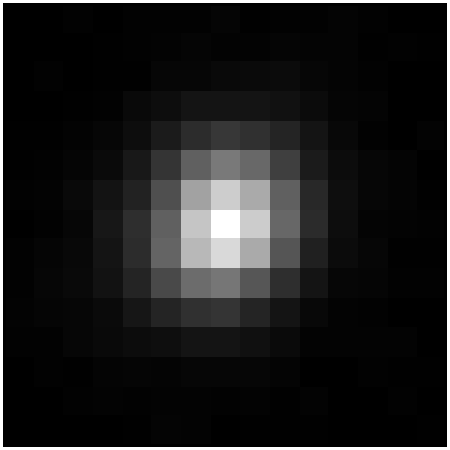
\includegraphics[height=0.22\textwidth]{psf-00}%
      }
      &&
      % gal img*
      \multicolumn{1}{r}{%
        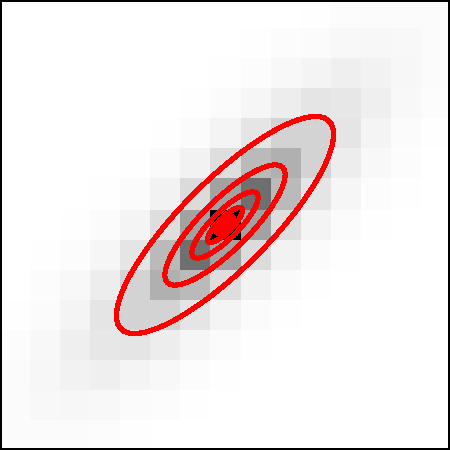
\includegraphics[height=0.22\textwidth]{psf-04}%
      }
      &&
      % psf * gal img
      \multicolumn{1}{r}{%
        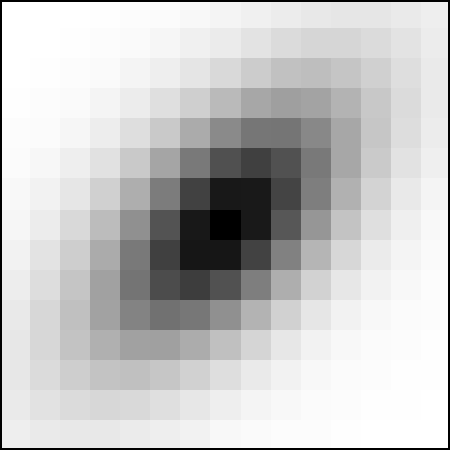
\includegraphics[height=0.22\textwidth]{psf-05}%
      } \\
      %
      \rule[-1em]{0pt}{1.5em}
      $\arrowspacer{\downarrow \mathcal{F}}$ && && $\arrowspacer{\uparrow \mathcal{F}^{-1}}$ \\
      %
      FFT(PSF) & $\times$ & FT(Galaxy) & $=$ & FFT(PSF $\conv$ Galaxy) \\
      % psf FT
      \multicolumn{1}{r}{%
        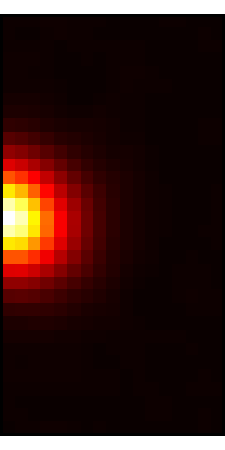
\includegraphics[height=0.22\textwidth]{psf-01}} &
      %$\times$
      &
      % gal FT
      \multicolumn{1}{r}{%
        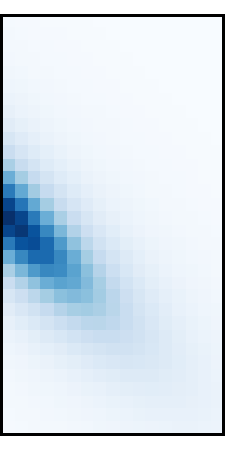
\includegraphics[height=0.22\textwidth]{psf-02}} &
      %$=$
      &
      % psf * gal FT
      \multicolumn{1}{r}{%
        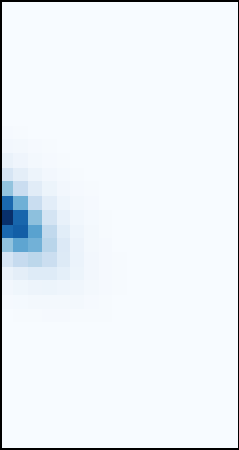
\includegraphics[height=0.22\textwidth]{psf-03}}
      % gal img
      %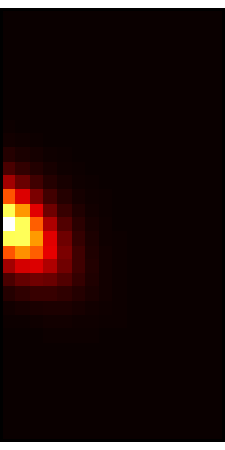
\includegraphics[height=0.22\textwidth]{psf-12} &
    \end{tabular}
  \end{center}
  \caption{\label{fig:example}%
    Illustration of the \trick.
    \textbf{Top-left}: pixelized PSF model (zoom-in of central region).
    %
    \textbf{Bottom-left}: FFT of the pixelized PSF model.  Since the PSF model is
    purely real, we show only half the symmetric Fourier transform. The FFT is
    complex; we show here the absolute value.
    % 
    \textbf{Top-middle}: pixel-space galaxy profile (which would be
    undersampled), with Gaussian ellipse approximations.  This is
    never evaluated in our method, and is shown only for illustration.
    % 
    \textbf{Bottom-middle}: the discrete Fourier-space representation of the
    galaxy profile, evaluated directly in Fourier space.
    %
    \textbf{Bottom-right}: product of the FFT of the PSF and the
    discrete Fourier transform of the galaxy model.
    %
    \textbf{Top-right}: the result: the galaxy model convolved by the
    PSF, in pixel space.  This is computed by inverse-FFT of the
    bottom-right panel.
  }
\end{figure}



% VERTICAL LAYOUT

\begin{figure}
  \newcommand{\arrowspacer}[1]{\left#1 \textrm{\rule[-0.5em]{0pt}{1em}} \right.}
  \begin{center}
    \begin{tabular}{@{}c@{}c@{}c@{}c@{}c@{}}
      %
      Pixel Space & 
      \rule{1ex}{0pt}
      & Fourier Space (Analytic) & & Fourier Space \\
      %
      %\hline \\
      \cline{1-1} \cline{3-3} \cline{5-5}
      %
      %Step 1: Pixel space PSF &   &   &   & Step 2 \\
      %
      Step 1: PSF &   &
      %$\Longrightarrow$FFT$\Longrightarrow$
        &
        &
      FFT(PSF) \\
      %
      % psf img
      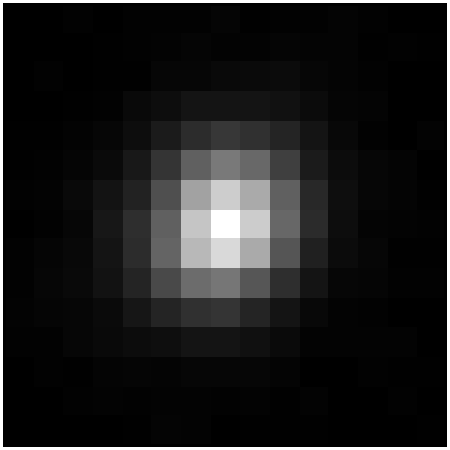
\includegraphics[height=0.22\textwidth]{psf-00}%
      &   & 
      %\raisebox{0.11\textwidth}{$-\negmedspace-$ FFT $\longrightarrow$}
      %
      % \raisebox{0.11\textwidth}{%
      %   $\xrightarrow{\displaystyle\textrm{\hspace{1em}
      %       Step 2: FFT \hspace{1em}}}$
      % }%
      \makebox[0em][c]{
        \raisebox{0.11\textwidth}{%
          \hspace{2em}$\xrightarrow{\displaystyle\textrm{\hspace{1em}
              Step 2: FFT \hspace{1em}}}$
        }%
      }
      %
      &   &
      % psf FT
      %\multicolumn{1}{r}{%
      \makebox[0.22\textwidth][r]{%
        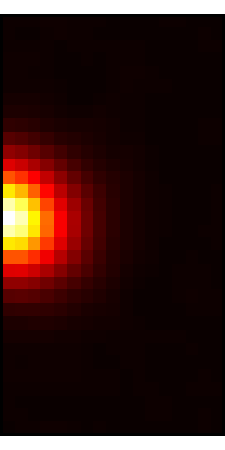
\includegraphics[height=0.22\textwidth]{psf-01}%
      }
      \\
      %
      %&   &   &   & $\times$ \\
      %
      Step 3: Galaxy MoG  &   & Step 4: FT(MoG) &   & Step 5: FT(Galaxy) \\
      %
      %\gray{Galaxy} &   &
      %Mixture of Gaussians &   &
      %FT(Galaxy) \\
      %
      % gal img
      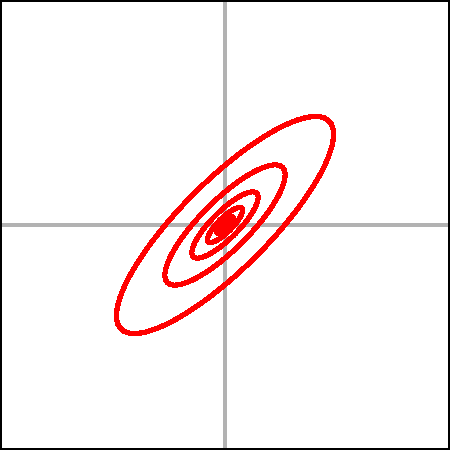
\includegraphics[height=0.22\textwidth]{psf-08}%
      & 
      &
      % gal analytic FT ellipses
      %\multicolumn{1}{r}{%
      %  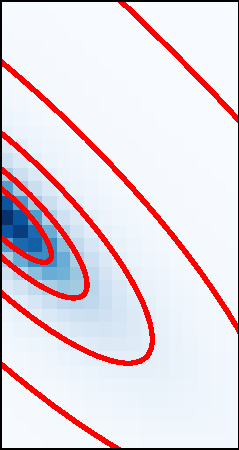
\includegraphics[height=0.22\textwidth]{psf-06}%
      %}%
      \makebox[0.22\textwidth][r]{%
        %\raisebox{0.11\textwidth}{\makebox[0ex][l]{$\longrightarrow$}}
        \raisebox{0.11\textwidth}{$\longrightarrow$}
        \hspace{1em}
        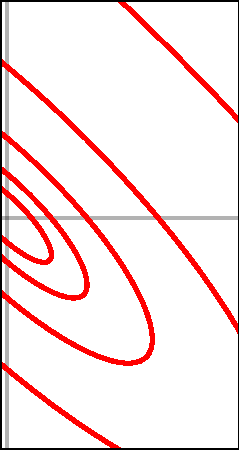
\includegraphics[height=0.22\textwidth]{psf-07}%
      }%
      &
      %\raisebox{0.11\textwidth}{$\rightarrow$}
      \raisebox{0.11\textwidth}{\makebox[1ex][l]{%
          \hspace{1em}$\longrightarrow$}}
      \
      &
      % gal FT
      %\multicolumn{1}{r}{%
      \makebox[0.22\textwidth][r]{%
        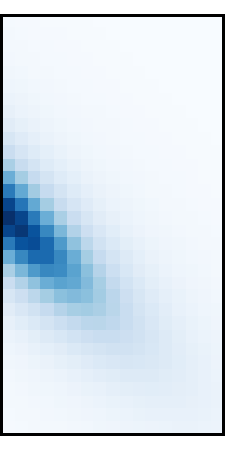
\includegraphics[height=0.22\textwidth]{psf-02}%
      }
      \\
      %
      %Step 6 &   &   &   & $=$ \\
      %
      PSF $\conv$ Galaxy &   &
        &   &
      FT(PSF $\conv$ Galaxy) \\
      %
      % psf * gal img
      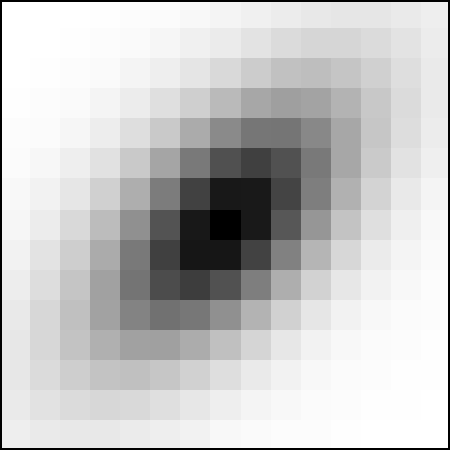
\includegraphics[height=0.22\textwidth]{psf-05}%
      &   &
      %\raisebox{0.11\textwidth}{$\longleftarrow$ FFT$^{-1}$ $ \longleftarrow$}
      %\raisebox{0.11\textwidth}{$\longleftarrow$ FFT$^{-1}$ $ \rule[1ex]{3ex}{1pt}$}
      %\raisebox{0.11\textwidth}{$\longleftarrow$ FFT$^{-1}$ $ -\negmedspace-$}
      %
       %\raisebox{0.11\textwidth}{%
       %  $\xleftarrow{\displaystyle%
       %    \textrm{\hspace{1em} Step 6: FFT$^{-1}$ \hspace{1em}}}$
       %}%
      \makebox[0em][c]{
        \raisebox{0.11\textwidth}{%
          \hspace{2em}$\xleftarrow{\displaystyle%
            \textrm{\hspace{1em} Step 6: FFT$^{-1}$ \hspace{1em}}}$
        }%
      }
      %
      &   &
      % psf * gal FT
      %\multicolumn{1}{r}{%
      \makebox[0.22\textwidth][r]{%
        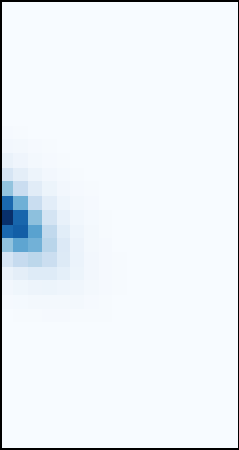
\includegraphics[height=0.22\textwidth]{psf-03}%
      }
      \\
      %
      %$\arrowspacer{\downarrow \mathcal{F}}$ && && $\arrowspacer{\uparrow \mathcal{F}^{-1}}$ \\
      %FFT(PSF) & $\times$ & FT(Galaxy) & $=$ & FFT(PSF $\conv$ Galaxy) \\
      %$\times$
      %\multicolumn{1}{r}{%
      % gal img
      %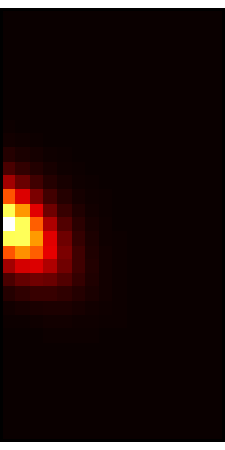
\includegraphics[height=0.22\textwidth]{psf-12} &
    \end{tabular}
  \end{center}
  \caption{\label{fig:example}%
    Illustration of the \trick.
    \textbf{Top-left}: pixelized PSF model (zoom-in of central region).
    %
    \textbf{Top-right}: 
    FFT of the pixelized PSF model.  Since the PSF model is
    purely real, we show only half the symmetric Fourier transform. The FFT is
    complex; we show here the absolute value.
    % 
    \textbf{Middle-left}: Pixel-space galaxy profile,
    Mixture-of-Gaussians (MoG) approximation.  The profile would be
    undersampled if evaluated in pixel space.
    % 
    \textbf{Middle}: The mixture-of-Gaussians galaxy approximation in
    Fourier space.
    %
    \textbf{Middle-right}: The discrete Fourier-space representation of the
    galaxy profile, evaluated directly in Fourier space.
    %
    \textbf{Bottom-right}: Product of the FFT of the PSF and the
    Fourier transform of the galaxy model.
    %
    \textbf{Bottom-left}: The result: the galaxy model convolved by the
    PSF, in pixel space.  This is computed by inverse-FFT of the
    bottom-right panel.
  }
\end{figure}





\section{The \Trick}

The \trick\ presented here builds directly upon our mixture-of-Gaussians
approximation of galaxy profiles, with the realization that the
Fourier transform of a Gaussian is also a Gaussian.  This allows us to
evaluate the Fourier transform of a model galaxy profile \emph{directly} in Fourier
space, without ever having to render the ``above the atmosphere''
(unconvolved) galaxy profile in pixel space.
% (which is problematic due to undersampling).
We can then multiply this Fourier-space
representation of the galaxy by the Fourier transform of the pixelized
PSF model, then inverse Fourier transform back to pixel space to get
the PSF-convolved galaxy profile.
%
As long as the pixelized PSF model is well sampled, this method produces
exact answers for each Gaussian in the mixture.

We will elaborate on each step of the \trick\ below.  In summary:
\begin{enumerate}
\item Choose the desired output image size and embed the pixelized PSF
  model in a zero-padded image of this size.
\item Compute the Fourier Transform of the padded PSF model via the
  Fast Fourier Transform (FFT),
  recording the frequencies $(v, w)$ of the FFT terms.
\item Transform the mixture-of-Gaussians approximation of the model
  galaxy through an ellipticity matrix and the local image World
  Coordinate System (WCS) matrix to get pixel-space Gaussians
  (also including sub-pixel shifts).
\item Convert the galaxy mixture-of-Gaussians from pixel space to Fourier space.
\item Evaluate the Fourier-space Gaussians on the frequency grid $(v, w)$.
\item Multiply the PSF and galaxy Fourier transforms and inverse-FFT
  back to pixel space.
\end{enumerate}
%We will elaborate on each step below.

The process is illustrated in Figure \ref{fig:example}.  Example code
is available alongside the paper source,\footnote{ Available at
  \niceurl{http://github.com/dstndstn/fft-gal-convolution}.}  and the
method is also implemented in \project{the Tractor} code.\footnote{%
  Available at
  \niceurl{http://github.com/dstndstn/tractor}.}

Step 1, choosing the desired output image size, depends on the size of
the PSF model as well as the galaxy.  If the chosen size is too small,
wrap-around will occur since the FFT is periodic; see Figure \ref{fig:wrap}.

In Step 2, we compute the FFT of the PSF.  If the PSF is constant
across the image, this FFT need only be computed once.  Alternatively,
some PSF modelling tools, including \project{PsfEx} \citep{psfex},
produce \emph{eigen-PSF} models.  That is, the PSF model varies
spatially across the image, and the variation is represented as
polynomial variations in the amplitudes of a set of PSF components.
This is convenient, since the FFT of each eigen-component can be
computed once in preprocessing and the FFT at a given position in the
image can be computed by weighting the component FFTs using the PSF
model's polynomial spatial variation terms.

In Step 3, we transform the mixture-of-Gaussians approximation of the
galaxy profiles from their representation in units of galaxy effective
radius into pixel units.  This includes an ellipse transformation
(scaling by effective radius, shearing by galaxy axis ratio, rotation
by galaxy position angle), plus a transformation into pixel
coordinates based on a locally-linear approximation of the image's
World Coordinate System.
% We split the pixel position of the galaxy center into integer and
% fractional parts.
The result is a pixel-space mixture-of-Gaussians representation of the
galaxy.

Specifically, in \project{the Tractor}, we represent the shape of a
galaxy by the effective radius $r_e$ and two ellipticity components
$e_1$ and $e_2$ as are typically used in weak lensing.  We can
represent this as a matrix that transforms from celestial coordinates
into units of effective radius (the coordinates in which the galaxy
profiles are written).  This is most easily done by computing the
position angle $\theta$ and axis ratio $a$,
\begin{align}
%
\theta & = \frac{1}{2} \arctan\!2(e_2, e_1) \\
%
e & = \sqrt{e_1^2 + e_2^2} \\
%
a & = \frac{1 - e}{1 + e} \label{eq:a}
\end{align}
leading to the transformation matrix
\begin{align}
E &= r_e \begin{bmatrix}
\textcolor{white}{-}a \cos{\theta} & \sin{\theta} \\
-a \sin{\theta} & \cos{\theta} \\
\end{bmatrix} \quad .
\end{align}
If we represent the local astrometric world coordinate system by an
affine transformation that takes celestial coordinates to pixel
coordinates, then we can multiply the two transformation matrices to
convert from pixels to galaxy profile coordinates.  The FITS WCS
standard \citep{wcs2} defines a transformation matrix $\CD$ that takes
pixels to intermediate world coordinates.  The combined transformation
matrix $T$ is then
\begin{align}
T & = (\CD)^{-1} E
\end{align}
so that a covariance matrix in galaxy effective radius coordinates can
be transformed into pixel space by computing
\begin{align}
C &= T \, V \, T^T
\label{eq:vpix}
\end{align}
where we will use isotropic variances $V = v I$.
When we write out this matrix in full, we find that the $\cos{\theta}$
and $\sin{\theta}$ terms always appear in pairs, so we can avoid
computing these trigonometric functions explicitly in the above.  See
\appref{app:transform}.


Step 4 is the core of the \trick.  The Fourier transform of
a Gaussian is another Gaussian; our mixture-of-Gaussian representation
of galaxy profiles can be converted into a mixture of Gaussians in
Fourier space.
%
A single 2-dimensional Gaussian
centered at the origin and
with covariance $C$
in pixel space is defined by
\begin{equation}
g(\bm{x}) = \frac{1}{2 \pi \sqrt{\det(C)}}
\exp\left( -\frac{1}{2} \bm{x}^T C^{-1} \bm{x} \right)
\end{equation}
which becomes, writing out the vector $\bm{x}$ as $(x,y)^T$
and symmetric covariance $C = \bigl(\begin{smallmatrix}
a&b \\ b&d
\end{smallmatrix} \bigr)$,
\begin{equation}
g(x, y) = \frac{1}{2 \pi \sqrt{a d - b^2}}
\exp \left(
-\frac{d x^2 - 2 b x y + a y^2}{2(a d - b^2)}
\right) \quad .
\end{equation}
%
The Fourier Transform of the shifted Gaussian $g(x - x_0, y - y_0)$ is defined as
\begin{equation}
G(v,w) =
\int\limits_{-\infty}^{\infty}
\int\limits_{-\infty}^{\infty}
g(x - x_0, y - y_0) e^{-2 \pi i (v x + w y)} \, \mathrm{d}x \, \mathrm{d}y
\quad .
\end{equation}
We use the shift theorem to move the centroid to $\mu = (x_0, y_0)$
in pixel space via a phase term in Fourier space;
\begin{equation}
G(v, w) =
e^{-2 \pi i (x_0 v + y_0 w)}
\int\limits_{-\infty}^{\infty}
\int\limits_{-\infty}^{\infty}
g(x, y) e^{-2 \pi i (v x + w y)} \, \mathrm{d}x \, \mathrm{d}y
\end{equation}
%
which, plugging in the covariance matrix $C$, works out to
\begin{equation}
G(v,w) =
e^{-2 \pi i (x_0 v + y_0 w)}
e^{-2 \pi^2 (a v^2 + 2 b v w + d w^2)}
\end{equation}
which can easily be evaluated on a grid of frequencies $(v, w)$.

For a mixture of Gaussians, we must evaluate $G$ for each component in
the mixture and compute their weighted sum.  In the case of a
mixture-of-Gaussians representation of affine-transformed galaxy
profiles, the centers $(x_0, y_0)$ are the same for each component in
the mixture; only the covariances,
$C_i = \bigl(\begin{smallmatrix}
a_i&b_i \\ b_i&d_i
\end{smallmatrix} \bigr)$,
differ.  The Fourier transform
of a mixture of Gaussians,
\begin{equation}
m(x,y) = \sum_i A_i \, g_i(x, y)
\end{equation}
is therefore
\begin{equation}
M(v, w) = e^{-2 \pi i (x_0 v + y_0 w)}
\sum_i A_i \,
e^{-2 \pi^2 (a_i v^2 + 2 b_i v w + d_i w^2)}
\quad .
\end{equation}



%%% Example of pushing our galaxy MOGs through a WCS, etc?


In Step 5 of our \trick, we directly evaluate these Gaussians in Fourier
space, on the same discrete frequency grid $(v, w)$ used for the FFT
of the PSF.  This has interesting properties.  By taking the Fourier
transform, we are effectively assuming that the PSF model is well
sampled, thus has zero power outside the frequency grid of the FFT.
The galaxy profile may have power outside that frequency range; this
is the reason that one cannot simply render the galaxy profile ``above
the atmosphere'' at the native image pixel scale and apply FFT
convolution na\"ively: In the limit, a point-like galaxy has power at
all frequencies.  But when we multiply the PSF and galaxy profile in
Fourier space, all that high-frequency power will be zeroed out by the
assumption of a well-sampled PSF model.  Effectively, by evaluating the
galaxy Fourier transform directly in the frequency space of the PSF
model, we are applying a perfect low-pass filter at exactly the
Nyquist limit.  By zeroing out the high-frequency power, we avoid the
aliasing that would otherwise result from Fourier transforming an
undersampled signal.
%

Finally, in Step 6, we multiply the PSF and galaxy Fourier transforms,
and apply the inverse FFT to return to pixel space.

\section{Discussion}

Our \trick\ is implemented in \project{the Tractor} code and has been
used at scale in the data reduction of the Dark Energy Camera Legacy
Survey Data Release 2 (Schlegel, Dey \etal, in prep.).  In our tests, we
have found the speed to be comparable to that of a 3-component
mixture-of-Gaussians representation of the PSF.  The majority of the
computational cost is in evaluating the \emph{exp} function rather
than in the FFT or inverse-FFT, so fast \emph{exp} approximations\footnote{%
For example, \niceurl{https://github.com/herumi/fmath} as used in
\project{ngmix}, \niceurl{https://github.com/esheldon/ngmix}.}
should provide significant speedups.

%http://homepage1.nifty.com/herumi/soft/fmath.html


\begin{figure}
\begin{center}
\begin{tabular}{@{}cc@{}}
  $256 \times 256$-pixel FFT &
  $32 \times 32$-pixel FFT \\
  %
  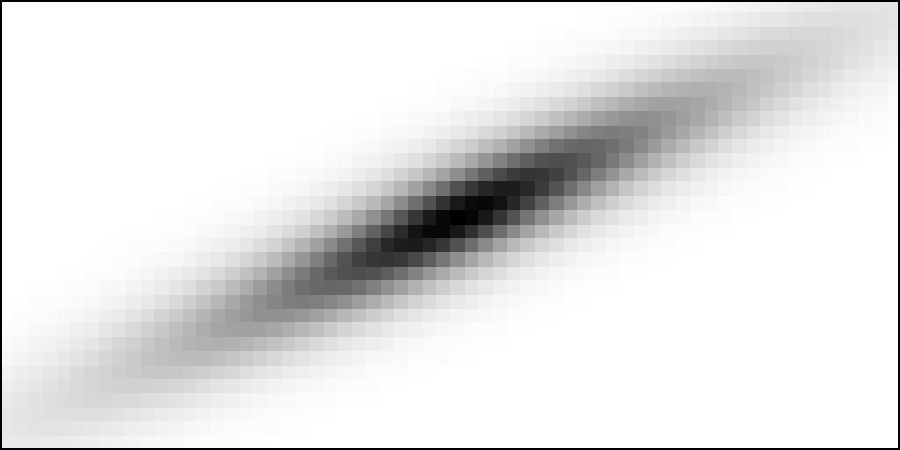
\includegraphics[height=0.22\textwidth]{gal-00} &
  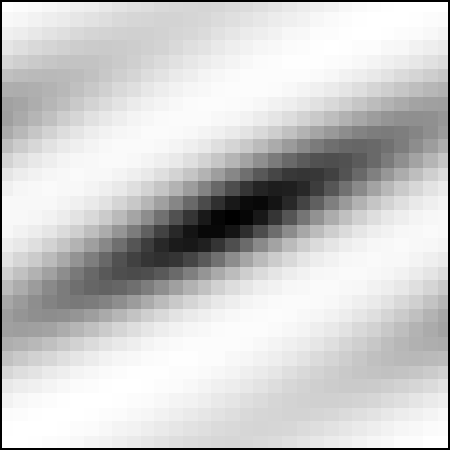
\includegraphics[height=0.22\textwidth]{gal-01} \\
\end{tabular}
\end{center}
\caption{\label{fig:wrap}%
  Wrap-around of the PSF-convolved galaxy profile can occur if the FFT is
  computed on a pixel grid too small to contain the galaxy.
  %
  \textbf{Left:} Result (cropped) using a 256-pixel square grid.
  %
  \textbf{Right:} Result using a 32-pixel square grid shows wrap-around
  aliasing.
}
\end{figure}

When using this \trick, one must choose the image patch size in which
to embed the PSF; the resulting convolved image will be the same size.
The image size chosen must be large enough to contain the convolved
galaxy, or wrap-around effects will be seen: The Fourier transform is
periodic, so any part of the convolved galaxy profile that lies
outside the image will alias into the image.  This is
illustrated in Figure \ref{fig:wrap}.



\acknowledgements

I thank Erin Sheldon (BNL),
David W.~Hogg (NYU), David J.~Schlegel (LBL), and John Moustakas (Siena)
for helpful discussion and comments on this manuscript.

The Dunlap Institute is funded through an endowment established by the
David Dunlap family and the University of Toronto.




\appendix

\section{Galaxy variances in pixel space}
\label{app:transform}

Writing out the matrix multiplication in \eqnref{eq:vpix} assuming an
isotropic variance $V = v I$, we get the pixel-space covariance matrix
\begin{align}
C = v f \begin{bmatrix}
C_{1,1} & C_{1,2} \\
C_{2,1} & C_{2,2}
\end{bmatrix}
\end{align}
where the matrix is symmetric so that $C_{1,2} = C_{2,1}$ and the terms are
\begin{align}
f & = \left( \frac{r_e}{t w - u v} \right)^2
\\
C_{1,1} & =
%
%a^2(w^2 c^2 + 2 u w c s + u^2 s^2) + w^2 s^2 - 2 u w c s + u^2 c^2
a^2(w^2 c^2 + 2 u w c s + u^2 s^2) + u^2 c^2 - 2 u w c s + w^2 s^2
\\
C_{1,2} & =
%
%-a^2 (v w c^2 + u v c s + t w c s + t u s^2) - v w s^2 + u v c s + t w c s - t u c^2
-a^2 (v w c^2 + (u v + t v) c s + t u s^2) - t u c^2 + (u v + t w) c s - v w s^2
\\
C_{2,2} & =
%
a^2 (v^2 c^2 + 2 t v c s + t^2 s^2) + t^2 c^2 - 2 t v c s + v^2 s^2
\end{align}
where $r_e$ is the galaxy effective radius in degrees,
$a$ is the axis ratio (\eqnref{eq:a}) and
we have defined the abbreviations
\begin{align}
\begin{bmatrix}
t & u \\
v & w
\end{bmatrix}
& = 
\begin{bmatrix}
\CD_{1,1} & \CD_{1,2} \\
\CD_{2,1} & \CD_{2,2}
\end{bmatrix}
=
\CD
\\
c &= \cos \theta \\
s &= \sin \theta
\end{align}
where the $\CD$ matrix terms have units of degrees per pixel.
Observe that the covariance terms only contain $c^2$, $cs$, and $s^2$
terms.  We can therefore use the identities:
\begin{align}
c^2 & = \cos^2 \theta            =
\tfrac{1}{2} \left(1 + \frac{e_1}{e} \right) \\
s^2 & = \sin^2 \theta            =
\tfrac{1}{2} \left(1 - \frac{e_1}{e} \right) \\
cs  & = \sin \theta \cos \theta  = %\tfrac{1}{2} \frac{e_2}{e}
\frac{e_2}{2 e}
\end{align}
where $e_1$ and $e_2$ are the two ellipticity components and $e =
\sqrt{e_1^2 + e_2^2}$.  This allows us to avoid computing $\theta$,
$\cos \theta$ and $\sin \theta$ explicitly when transforming a galaxy
into pixel space.

% NO we still need $a$
% In \project{the Tractor} we find this particularly useful because we
% use a ``softened'' remapping of the ellipticity components to avoid
% the hard edges in parameter space $\|e\| < 1$.  Since the pixel-space
% covariance matrix can be computed using only 

For convenience, we repeat here the mixture-of-Gaussians fits for the
SDSS truncated exponential and deVaucouleurs profiles that we use in
\project{the Tractor}:
\begin{center}
\begin{tabular}{cr@{.}lr@{.}lr@{.}lr@{.}l}
\hline
\textbf{Component} &
\multicolumn{4}{c}{\textbf{Exponential}} & 
\multicolumn{4}{c}{\textbf{deVaucoulers}} \\
& \multicolumn{2}{c}{Amplitude}
& \multicolumn{2}{c}{Variance}
& \multicolumn{2}{c}{Amplitude}
& \multicolumn{2}{c}{Variance} \\
\hline
1 & 
$1$ & $99485977 \times 10^{-4}$
&
$1$ & $20078965 \times 10^{-3}$
&
$2$ & $01837690 \times 10^{-3}$
&
$2$ & $23759216 \times 10^{-4}$
\\
%
2 &
$2$ & $61612679 \times 10^{-3}$
&
$8$ & $84526493 \times 10^{-3}$
&
$1$ & $13678862 \times 10^{-2}$
&
$1$ & $00220099 \times 10^{-3}$
\\
%
3 &
$1$ & $89726655 \times 10^{-2}$
&
$3$ & $91463084 \times 10^{-2}$
&
$3$ & $24716253 \times 10^{-2}$
&
$4$ & $18731126 \times 10^{-3}$
\\
%
4 &
$1$ & $00186544 \times 10^{-1}$
&
$1$ & $39976817 \times 10^{-1}$
&
$7$ & $19288205 \times 10^{-2}$
&
$1$ & $69432589 \times 10^{-2}$
\\
%
5 &
$3$ & $68534484 \times 10^{-1}$
&
$4$ & $60962500 \times 10^{-1}$
&
$1$ & $34272271 \times 10^{-1}$
&
$6$ & $84850479 \times 10^{-2}$
\\
%
6 &
$5$ & $09490694 \times 10^{-1}$
&
$1$ & $50159566$
&
$2$ & $11362649 \times 10^{-1}$
&
$2$ & $87207080 \times 10^{-1}$
\\
%
7 &
\multicolumn{2}{c}{-} &
\multicolumn{2}{c}{-} &
$2$ & $70999815 \times 10^{-1}$
&
$1$ & $33320254$
\\
%
8 &
\multicolumn{2}{c}{-} &
\multicolumn{2}{c}{-} &
$2$ & $65578557 \times 10^{-1}$
&
$8$ & $40215071$
\\
\hline
\end{tabular}
\end{center}
Fits for other numbers of mixture components are available in
\cite{moggalaxy}.  The code used to compute these values is publicly
available at \niceurl{http://github.com/davidwhogg/TheTractor}.

\begin{thebibliography}

\bibitem[Berg\'e \etal(2013)]{ufig}
Berg\'e,~J. \etal, 2013, Astronomy and Computing, 1, 23;
\arxiv{1209.1200}
% An Ultra Fast Image Generator (UFig) for wide-field astronomy


\bibitem[Bertin (2011)]{psfex}
Bertin, E., 2011, ADASS XX, ASP Conference Series, 442, 435
%Evans, I.~N., Accomazzi, A., Mink, D.~J. and Rots, A.~H., eds.

\bibitem[Calabretta \& Greisen(2002)]{wcs2}
Calabretta,~M.~R. \& Greisen,~E.~W., 2002, 
%\AA,
Astronomy \& Astrophysics, 
395, 1077;
\arxiv{astro-ph/0207413}

\bibitem[Hogg \& Lang(2013)]{moggalaxy}
Hogg,~D.~W. \& Lang,~D., 2013, \pasp, 125, 719;
\arxiv{1210.6563}

% Detailed Structural Decomposition of Galaxy Images
\bibitem[Peng \etal(2002)]{galfit}
 Peng,~C.~Y. \etal, 2002, \aj, 124, 266;
 \arxiv{0204182}

% PhoSim: a code to simulate telescopes one photon at a time
%Peterson,~J.~R., 2014, Journal of Instrumentation, 9, C04010;

%Simulation of Astronomical Images from Optical Survey Telescopes using a Comprehensive Photon Monte Carlo Approach
\bibitem[Peterson \etal(2015)]{phosim}
Peterson,~J.~R. \etal, 2015, \apjs, 218, 14;
\arxiv{1504.06570}

\bibitem[Rowe \etal(2015)]{galsim}
  Rowe,~B. \etal, 2015, Astronomy and
  Computing, 10, 121; \arxiv{1407.7676}
% GalSim: The modular galaxy image simulation toolkit

\bibitem[Sheldon (2014)]{ngmix}
  Sheldon,~E.~S., 2014, MNRAS, 444, 25;
  \arxiv{1403.7669}

\end{thebibliography}


\end{document}
